

\documentclass[t]{beamer}
\usetheme{Antibes}% theme
\usepackage{mwe}
\usepackage{xcolor}
\usepackage{amsmath,amsfonts,amssymb} % This makes the equations appears better
\usepackage{animate}
\usepackage{ragged2e}
\usecolortheme{spruce}

\apptocmd{\frame}{}{\justifying}{}
\setbeamertemplate{navigation symbols}{}


\usepackage{amsmath}
\usepackage{bm}
%\newcommand{\uveci}{{\bm{\hat{\textnormal{\bfseries\i}}}}}
%\newcommand{\uvecj}{{\bm{\hat{\textnormal{\bfseries\j}}}}}
%\DeclareRobustCommand{\uvec}[1]{{%
%  \ifcsname uvec#1\endcsname
%     \csname uvec#1\endcsname
%   \else
%    \bm{\hat{\mathbf{#1}}}%
%   \fi
%}}

\usepackage{bm}
\newcommand{\uveck}{\bm{\hat{k}}}
\newcommand{\uveci}{\bm{\hat{\imath}}}
\newcommand{\uvecj}{\bm{\hat{\jmath}}}

\newcommand{\fillend}{\vskip0pt plus 1filll}

\newcommand\Tstrut{\rule{0pt}{2.6ex}}         % = `top' strut
\newcommand\Bstrut{\rule[-0.9ex]{0pt}{0pt}}   % = `bottom' strut
%%%%%%%%%%%%%%%%%%%%%%%%%%%%%%%%%%%%%%%%%%%%%%%%%%%%%%%%%%%%%%%%%%%%%%%%%%%%%%



%\author[Enrique Wagemann]{\normalsize Dr. Enrique Wagemann \newline \small{ewagemann@udec.cl}}

%\institute[Universidad de Concepci\'{o}n]{\textcolor{black}{Facultad de Ingenier\'{i}a - Departamento de Ingenier\'{i}a Mec\'{a}nica \and Universidad de Concepci\'{o}n}}

\setbeamertemplate{headline}
{%
  \leavevmode%
 \begin{beamercolorbox}[wd=.5\paperwidth,ht=2.5ex,dp=1.125ex]{section in head/foot}%
    \hbox to .5\paperwidth{\hfil\insertsectionhead\hfil}
  \end{beamercolorbox}%
  \begin{beamercolorbox}[wd=.5\paperwidth,ht=2.5ex,dp=1.125ex]{subsection in head/foot}%
    \hbox to .5\paperwidth{\hfil\insertsubsectionhead\hfil}
  \end{beamercolorbox}%
}

\makeatletter
\newcommand\titlegraphicii[1]{\def\inserttitlegraphicii{#1}}
\titlegraphicii{}
\setbeamertemplate{title page}
{
  \begin{centering}
  	\vspace{2.0cm}

	\usebeamerfont{title}\inserttitle\par%
	\vspace{0.6cm}

	\huge\insertsubtitle\par%

	\vspace{2.5cm}
    \begin{beamercolorbox}[sep=4pt,center]{author}
    \usebeamerfont{author}\insertauthor
    \end{beamercolorbox}


    %\end{beamercolorbox}%
    \vskip1em\par
%vspace
\vspace{0.7cm}
	%%%%%%%%% date%%%%%%%%%%
	\begin{beamercolorbox}[sep=8pt,center]{date}
	\usebeamerfont{date}\insertdate
	\end{beamercolorbox}%\vskip0.5em
  \end{centering}
  %\vfill
}
\makeatother


\begin{document}

\begin{frame}[plain]

\vspace{0.5cm}
\begin{minipage}{0.1\linewidth}
{\flushleft
\includegraphics[height=1.5
cm]{FI} }
\end{minipage}\hfill
\centering\begin{minipage}{0.55\linewidth}
\end{minipage}\hfill
\begin{minipage}{0.2\linewidth}
\flushright

\includegraphics[height=1.5cm]{udec}
\end{minipage}
\vspace{-1.5cm}

\centering\scriptsize{Facultad de Ingenier\'ia}

\centering\scriptsize{Universidad de Concepci\'on}


\title[\today]{{\textbf{\huge{MEC\'ANICA DE FLUIDOS}}}}

\subtitle[\today]{\textbf{\textcolor{black}{5 - Análisis dimensional}}}

\maketitle


\end{frame}



%%%%%%%%%%%%%%%%%%%%%%%%%%%%%%%%%%%%%%%%%%%%%%%%%%%%%%%%%%%%%%%%%%%%%%%%%%%%%%
%%%%%%%%%%%%%%%%%%%%%%%%%%%%%%%%%%%%%%%%%%%%%%%%%%%%%%%%%%%%%%%%%%%%%%%%%%%%%%
%%%%%%%%%%%%%%%%%%%%%%%%%%%%%%%%%%%%%%%%%%%%%%%%%%%%%%%%%%%%%%%%%%%%%%%%%%%%%%
%%%%%%%%%%%%%%%%%%%%%%%%%%%%%%%%%%%%%%%%%%%%%%%%%%%%%%%%%%%%%%%%%%%%%%%%%%%%%%

\section{Análisis dimensional}
\subsection{Introducción}
\begin{frame}[c]
\frametitle{Análisis dimensional}

En este capítulo exploraremos la técnica de \textbf{análisis dimensional}, la cual (a groso modo) consiste en el uso de parámetros adimensionales para la descripción de procesos físicos. Esta técnica permitirá analizar problemas que pudieran ser muy complejos para las técnicas de análisis integral o diferencial y se basa en la agrupación de las variables (o parámetros), mediante su multiplicación o cociente, en grupos que se caracterizan por carecer de dimensiones (dicho de otra forma, por ser adimensionales). Esta agrupación resulta en una disminución efectiva de la cantidad de parámetros requeridos para modelar el fenómeno en cuestión y, por ende, simplificando el problema a estudiar. Además, si se realiza de manera correcta, permitirá plantear, interpretar, presentar y extrapolar resultados experimentales.


\end{frame}

\begin{frame}[c]
\frametitle{Resultados de aprendizaje}

\begin{Large}
{\textbf{R8:	 Proponer modelos a escala para abordar diferentes problemas de mecánica de fluidos a partir del análisis dimensional.}}
\end{Large}

\end{frame}

%%%%%%%%%%%%%%%%%%%%%%%%%%%%%%%%%%%%%%%%%%%%%%%%%%%%%%%%%%%%%%%%%%%%%%%%%%%%%%
\begin{frame}[c]
\frametitle{Objetivo de la clase}

{\textbf{
\begin{itemize}
\item Reconocer los principios del análisis dimensional
\item Aplicar el teorema pi de Buckingham para generar parámetros adimensionales
\item Reconocer grupos adimensionales relevantes para la mecánica de fluidos
\end{itemize}
}}

\end{frame}

%%%%%%%%%%%%%%%%%%%%%%%%%%%%%%%%%%%%%%%%%%%%%%%%%%%%%%%%%%%%%%%%%%%%%%%%%%%%%%
\subsection{Dimensiones}
\begin{frame}
\frametitle{Dimensiones}
\textbf{Dimensión: medida con la que una magnitud física es expresada cuantitativamente.}
\vspace{0.2cm}

En este curso utilizaremos el sistema $\mathrm{\color{red}{MLtT}}$, consistente de $4$ dimensiones básicas:
\vspace{-0.5cm}

\begin{columns}
\column{0.5\textwidth}
\begin{itemize}
\item Tiempo ($\mathrm{t}$)
\item Longitud ($\mathrm{L}$)
\end{itemize}

\column{0.5\textwidth}
\begin{itemize}
\item Masa ($\mathrm{M}$)
\item Temperatura ($\mathrm{T}$)
\end{itemize}

\end{columns}
\vspace{0.5cm}

\textbf{Ejemplos:}
\vspace{-0.5cm}

\begin{columns}
\column{0.5\textwidth}
\begin{itemize}
\item Fuerza
\vspace{-0.5cm}

$$[F] = \mathrm{MLt^{-2}}$$
\vspace{-0.6cm}

\item Viscosidad
\vspace{-0.5cm}

$$[\mu] = \mathrm{ML^{-1}t^{-1}}$$
\vspace{-0.6cm}

\item Viscosidad cinemática
\vspace{-0.5cm}

$$[\nu] = \mathrm{L^{2}t^{-1}}$$

\end{itemize}

\column{0.5\textwidth}

\begin{itemize}
\item Velocidad
\vspace{-0.5cm}

$$[v] =\mathrm{ Lt^{-1}}$$
\vspace{-0.6cm}

\item Flujo másico
\vspace{-0.5cm}

$$[\dot{m}] = \mathrm{Mt^{-1}}$$
\vspace{-0.6cm}
\item Flujo volumétrico
\vspace{-0.5cm}

$$[Q] = \mathrm{L^3t^{-1}}$$



\end{itemize}

\end{columns}
\end{frame}

%%%%%%%%%%%%%%%%%%%%%%%%%%%%%%%%%%%%%%%%%%%%%%%%%%%%%%%%%%%%%%%%%%%%%%%%%%%%%%
\subsection{Principio de homogeneidad dimensional}
\begin{frame}
\frametitle{Principio de homogeneidad dimensional}
\small
\begin{itemize}
\item Una ecuación deducida analíticamente que representa un fenómeno físico debe ser válida para todos los sistemas de unidades.
\item Cada t\'ermino aditivo en la ecuaci\'on debe tener las mismas dimensiones.
\item La ecuaci\'on es valida en cualquier sistema de unidades.
\item La integraci\'on o diferenciaci\'on de la ecuaci\'on cambiara su dimensionalidad, mas no su homogeneidad.
\end{itemize}
\vspace{0.2cm}

\begin{small}

 \textbf{Ejemplo}: Posici\'on de un cuerpo en caida libre:
\begin{equation}
y=y_0+v_0t+\frac{1}{2}gt^2
\end{equation}
\vspace{-0.9cm}

\begin{columns}[c]
\column{0.5\textwidth}
\begin{itemize}
\item $[y] = [y_0] =  \mathrm{L}$
\item $[v_0]=\mathrm{Lt^{-1}} $
\item $[t]=\mathrm{t}$
\item $[g]=\mathrm{Lt^{-2}} $
\end{itemize}
\column{0.5\textwidth}
$$[y] = [y_0] = [v_0t] = \left[\frac{1}{2}gt^2\right]  = L$$
\end{columns}
\end{small}
\end{frame}


%%%%%%%%%%%%%%%%%%%%%%%%%%%%%%%%%%%%%%%%%%%%%%%%%%%%%%%%%%%%%%%%%%%%%%%%%%%%%%

\section{Grupos adimensionales}
\begin{frame}
\frametitle{Grupos adimensionales}
Los \textbf{grupos adimensionales} corresponden a grupos de cantidades \textbf{cuyo cociente o producto carece de dimensiones}.

\vspace{0.5cm}

\textbf{Ejemplo:} Número de Reynolds ($\operatorname{Re}$)


$$\mathrm{Re} = \frac{\rho V L}{\mu}$$

Podemos comprobar fácilmente que  es efectivamente adimensional, al analizar las dimensiones de cada uno de sus términos:
$$[\operatorname{Re}]=\frac{\color{red}{[\rho]}\color{blue}{[V]}\color{green}{[L]}}{\color{magenta}{[\mu]}}=\mathrm{\frac{\color{red}{\frac{M}{L^{3}}}\color{blue}{\frac{L}{t}}\color{green}{L}}{\color{magenta}{\frac{M}{L t}}}}=[1]$$
\end{frame}


%%%%%%%%%%%%%%%%%%%%%%%%%%%%%%%%%%%%%%%%%%%%%%%%%%%%%%%%%%%%%%%%%%%%%%%%%%%%%%

\section{Principios del análisis dimensional}
\begin{frame}
\frametitle{Principios del análisis dimensional}
Analicemos los principios del análisis dimensional y su importancia mediante el siguiente ejemplo: \textbf{Deseamos determinar la fuerza que se ejerce sobre una esfera sumergida en un campo de flujo.}
\begin{columns}[c]
\column{0.5\textwidth}
\begin{figure}
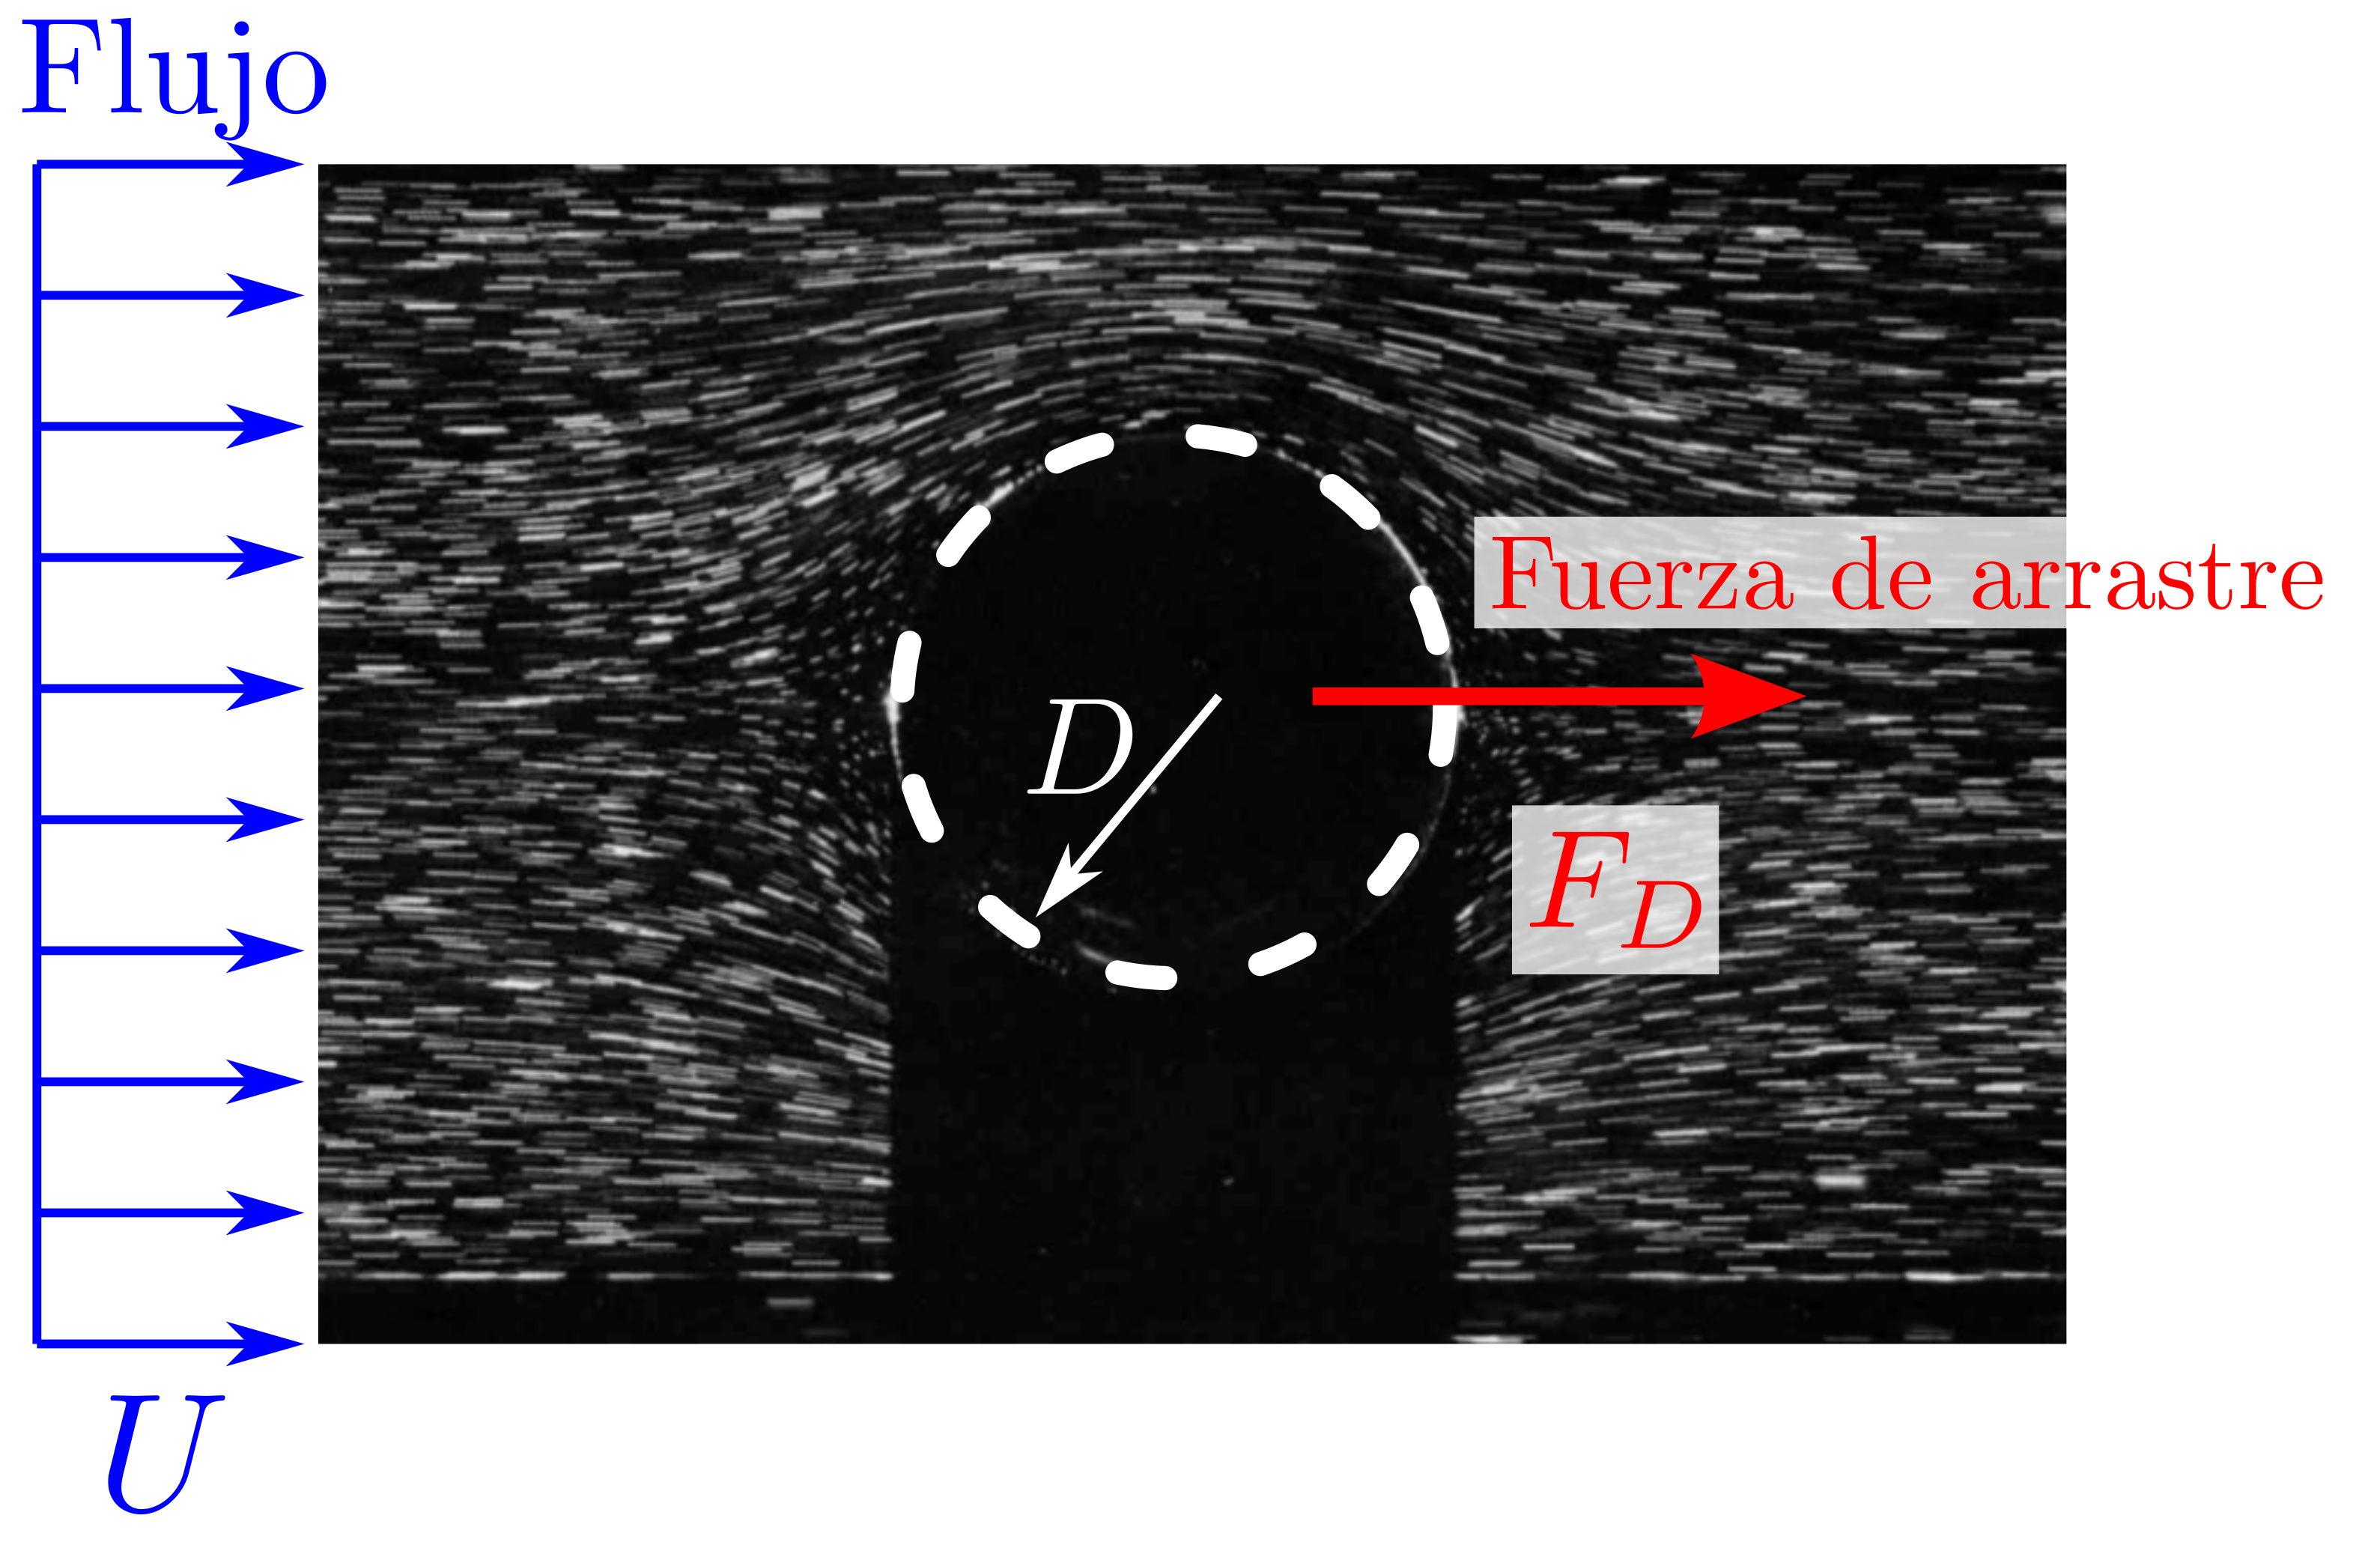
\includegraphics[width=1\textwidth]{Figures/Stokes_sphere.png}
\end{figure}
\column{0.5\textwidth}
{\justifying{Analíticamente, podemos determinar esta fuerza para flujos con velocidades muy pequeñas (flujos reptante):}}

$$F_ D =   3\pi\mu U D$$

{\justifying{\textbf{Sin embargo, a medida que la velocidad aumenta, este análisis se vuelve muy complejo \color{red}{(¡incluso imposible!)}}}}

\end{columns}
\end{frame}

%%%%%%%%%%%%%%%%%%%%%%%%%%%%%%%%%%%%%%%%%%%%%%%%%%%%%%%%%%%%%%%%%%%%%%%%%%%%%%
\begin{frame}
\textbf{Propuesta}: Ya que un análisis teórico no será posible, {\color{red}{investiguemos experimentalmente el flujo alrededor de la esfera}} \textbf{(pero antes, ¡debemos planificar nuestros experimentos!)}
\vspace{0.5cm}

Previo a diseñar nuestros experimentos, consideremos los parámetros que supondremos tendrán un efecto importante sobre la fuerza de arrastre:

\begin{itemize}
\item Velocidad del flujo ($U$)
\item Diámetro de la esfera ($D$)
\item Propiedades del fluido:
\begin{itemize}
\item Viscosidad ($\mu$)
\item Densidad ($\rho$)
\end{itemize}
\end{itemize}

De esta forma, podremos inicialmente suponer que la fuerza de arrastre $F_D$ será una función de $U$, $D$, $\mu$ y $\rho$:

$$F_D = f\left(U, D, \rho, \mu\right)$$

\end{frame}

\begin{frame}
Ahora, diseñemos nuestros experimentos:
\begin{small}

\begin{columns}[c]
\column{0.5\textwidth}
\begin{enumerate}
\justifying
\item Iniciemos con \textbf{$10$ mediciones} independientes sobre una esfera de diametro fijo en un tunel de viento, en las que variamos la  \textbf{velocidad} del flujo.
\item Analicemos ahora el efecto del diámetro de la esferza (supongamos que \textbf{mediciones sobre esferas de $10$ diámetros distintos} bastan)
\end{enumerate}
\column{0.5\textwidth}
\textbf{\color{red}{¿Existe un efecto cruzado entre diámetro y velocidad?}}
\begin{itemize}
\item Deberemos realizar las $10$ mediciones de velocidad sobre cada una de las $10$ esferas \textbf{(En total, $100$ experimentos)}
\end{itemize}
\end{columns}
\vspace{0.2cm}

Sumemos ahora el posible efecto de la \textbf{viscosidad} y \textbf{densidad} (que podremos caracterizar con $10$ corridas experimentales para cada propiedad)
\end{small}
\vspace{0.5cm}

{\centering{$\Rightarrow$ {\color{red}{\textbf{¡Deberemos realizar $\mathbf{10000}$ corridas experimentales para caracterizar nuestro flujo!}}}}}
\end{frame}

%%%%%%%%%%%%%%%%%%%%%%%%%%%%%%%%%%%%%%%%%%%%%%%%%%%%%%%%%%%%%%%%%%%%%%%%%%%%%%
\begin{frame}[t]
\begin{small}

\textbf{Propuesta alternativa}: Al realizar un análisis dimensional descubriremos que los parámetros que caracterizan nuestro flujo ($F_D$, $U$, $\rho$, $\mu$, $D$) se relacionan mediante la siguiente expresión:

$${\color{red}{\frac{F_D}{\rho U^2 D^2}}} = f\,^\prime\,\left({\color{blue}{\frac{\rho U D}{\mu}}}\right)$$

\begin{columns}[T]
\column{0.6\textwidth}
{\color{red}{Si multiplicamos el término en rojo por $8\pi$ obtendremos el coeficiente de arrastre $C_D$ (que corresponde a un grupo adimensional):}}

$$
\color{red}{C_{D}=\frac{F}{\frac{1}{2} \rho U^{2} \frac{\pi}{4} D^{2}}}
$$

\column{0.4\textwidth}

{\color{blue}{El término en azul corresponde al número de Reynolds:}}

$$\color{blue}{\operatorname{Re}= \frac{\rho U D}{\mu}}$$
\end{columns}
De esta forma:


$$C_D = f\,^\prime(\operatorname{Re})$$


\begin{center}
\textbf{\color{red}{¡Hemos reducido nuestro problema a dos parámetros!}}
\end{center}
\end{small}

\begin{footnotesize}
Esta reducción de parámetros sugiere que podemos reducir el número de experimentos considerablemente, ya que exiten menos variables que debemos considerar
\end{footnotesize}
\end{frame}
%%%%%%%%%%%%%%%%%%%%%%%%%%%%%%%%%%%%%%%%%%%%%%%%%%%%%%%%%%%%%%%%%%%%%%%%%%%%%%
\section{Teorema Pi de Buckingham}
\begin{frame}
\frametitle{Teorema Pi de Buckingham}

El \textbf{teorema Pi de Buckingham} permite determinar una relación entre grupos adimensionales, reduciendo efectivamente el número de variables involucradas y simplificando el problema a estudiar.
\vspace{0.2cm}

Este teorema se divide en dos partes:

\begin{itemize}

\item Si un proceso físico satisface el principio de homogeneidad dimensional e involucra $n$ variables, entonces \textbf{puede ser reducido a una relación entre solo $k$ variables adimensionales o $\Pi$s}. La reducción $j=n-k$ será igual al máximo número de variables que no forman un pi entre ellas y siempre es menor o igual que el número de dimensiones que describen las variables
\end{itemize}

\begin{columns}
\column{0.7\textwidth}
\begin{footnotesize}
\vspace{-0.4cm}

En nuestro problema de la esfera:

\begin{itemize}
\item Existen $5$ variables ($F$, $D$, $\mu$, $\rho$ y $U$)
\item Las variables están descritas por $3$ dimensiones ($\mathrm{M}$, $\mathrm{L}$ y $\mathrm{t}$)
\end{itemize}  

\end{footnotesize}
\column{0.3\textwidth}
$$k = n-j\geq 5-3 = 2$$
\end{columns}

\end{frame}
%%%%%%%%%%%%%%%%%%%%%%%%%%%%%%%%%%%%%%%%%%%%%%%%%%%%%%%%%%%%%%%%%%%%%%%%%%%%%%


\begin{frame}
\begin{itemize}
\item Encontrar la reducción $j$ y después seleccionar $j$ variables que no formen un pi entre ellas. Cada grupo pi deseado será una potencia del producto de estas $j$ variables más una variable adicional, a la cual se le asigna cualquier exponente distinto a cero. Cada grupo pi encontrado será independiente.
\end{itemize}
\end{frame}
%%%%%%%%%%%%%%%%%%%%%%%%%%%%%%%%%%%%%%%%%%%%%%%%%%%%%%%%%%%%%%%%%%%%%%%%%%%%%%

\section{Aplicación del teorema Pi de Buckingham}
\begin{frame}
\frametitle{Aplicación del teorema Pi de Buckingham}
El teorema Pi de Buckingham puede ser convenientemente dividido en $7$ pasos {\color{red}{(en rojo, la aplicación al ejemplo discutido en la sección anterior)}}

\begin{enumerate}
\item \textbf{Contar y hacer una lista con las $n$ variables involucradas en el problema}\newline
{\color{red}{En el ejemplo anterior existen 5 variables: $F$, $D$, $\mu$, $\rho$ y $U$.}}
\item \textbf{Seleccionar un conjunto de dimensiones primarias}\newline
{\color{red}{Las dimensiones primarias son: $\mathrm{M}$, $\mathrm{L}$ y $\mathrm{t}$ }}
\item \textbf{Hacer una lista con las dimensiones de cada variable}
$$\color{red}{\begin{array}{c|rrrrr} 
& F & U & D & \rho & \mu \\
\hline \mathrm{M} & 1 & 0 & 0 & 1 & 1 \\
\mathrm{L} & 1 & 1 & 1 & -3 & -1 \\
\mathrm{t} & -2 & -1 & 0 & 0 & -1
\end{array}}
$$
\end{enumerate}

\end{frame}
%%%%%%%%%%%%%%%%%%%%%%%%%%%%%%%%%%%%%%%%%%%%%%%%%%%%%%%%%%%%%%%%%%%%%%%%%%%%%%
\begin{frame}
\begin{enumerate}
\setcounter{enumi}{3}
\item \textbf{Encontrar la reducción $j=n-k$}\newline
{\color{red}{Matriz dimensional del proceso (notar que se obtiene a partir de la tabla desarrollada en el paso anterior):}}
$$\color{red}{\left(\begin{array}{rrrrr}1 & 0 & 0 & 1 & 1 \\ 1 & 1 & 1 & -3 & -1 \\ -2 & -1 & 0 & 0 & -1\end{array}\right)}$$  
{\color{red}{La reducción $j$ será equivalente al rango de la matriz dimensional:}}
$$\color{red}{\left|\begin{array}{rrr}1 & 0 & 0 \\ 1 & 1 & 1 \\ -2 & -1 & 0\end{array}\right|=1 \neq 0 \rightarrow \text{ El rango de la matriz es }3 \rightarrow j=3}$$
\end{enumerate}
\end{frame}
%%%%%%%%%%%%%%%%%%%%%%%%%%%%%%%%%%%%%%%%%%%%%%%%%%%%%%%%%%%%%%%%%%%%%%%%%%%%%%
\begin{frame}
\begin{enumerate}
\setcounter{enumi}{4}
\item \textbf{Seleccionar un grupo de j variables, las cuales (en conjunto) contengan todas las dimensiones primarias.}
\begin{small}
\begin{itemize}
\item Estas variables serán combinados con cada uno de los parámetros restantes (uno a la vez), por lo que son denominadas como variables de repetición
\item Las dimensiones de las variables de repetición seleccionadas no pueden ser obtenidas mediante potencias de otras variables de repetición
\item No seleccionar el parámetro dependiente como variable de repetición
\end{itemize}
{\color{red}Variables de repetición $\rho$, $U$  y $D$}
\end{small}

\end{enumerate}
\end{frame}
%%%%%%%%%%%%%%%%%%%%%%%%%%%%%%%%%%%%%%%%%%%%%%%%%%%%%%%%%%%%%%%%%%%%%%%%%%%%%%
\begin{frame}
\begin{enumerate}
\setcounter{enumi}{5}
\item \textbf{Armar ecuaciones dimensionales, combinando los parámetros seleccionados en el paso anterior con el resto de los parámetros. Resolver las ecuaciones dimensionales para obtener los $k$ grupos adimensionales.}
\end{enumerate}
$$\color{red}{\Pi_{1}=\rho^{a} U^{b} D^{c} F \rightarrow\left(\frac{M}{L^{3}}\right)^{a}\left(\frac{L}{t}\right)^{b}(L)^{c}\left(\frac{M L}{t^{2}}\right)=\left(M^{0} L^{0} t^{0}\right)}$$
\color{red}{Igualando los exponentes para cada dimensión:}
$$\color{red}{\begin{array}{rrcc}
M:& a+1=0 & & a=-1 \\
L:& -3a+b+c+1=0 & \rightarrow & c=-2\\
t:& -b-2=0 & & b=-2
\end{array}}
$$     
{\color{red}{Entonces:}}
$$
\color{red}{\Pi_{1}=\frac{F}{\rho U^{2} D^{2}}}
$$
\end{frame}

%%%%%%%%%%%%%%%%%%%%%%%%%%%%%%%%%%%%%%%%%%%%%%%%%%%%%%%%%%%%%%%%%%%%%%%%%%%%%%
\begin{frame}
\frametitle{}
{\color{red}{El segundo grupo adimensional se construye de igual forma:}}
$$\color{red}{
\Pi_{2}=\rho^{d} U^{e} D^{f} \mu \rightarrow\left(\frac{M}{L^{3}}\right)^{d}\left(\frac{L}{t}\right)^{e}(L)^{f}\left(\frac{M}{Lt}\right)=\left(M^{0} L^{0} t^{0}\right)
}$$
    
$$\color{red}{
\begin{array}{rr}
M: & d+1=0 \\
L: & -3 d+e+f-1=0 \\
t: & -e-1=0
\end{array}\quad \rightarrow\quad \begin{aligned}
d &=-1 \\
f & =-1 \\
e &= -1
\end{aligned}
}$$

{\color{red}{Entonces:}}

$$\color{red}{
\Pi_{2}=\frac{\mu}{\rho U D}
}$$  
\end{frame}

%%%%%%%%%%%%%%%%%%%%%%%%%%%%%%%%%%%%%%%%%%%%%%%%%%%%%%%%%%%%%%%%%%%%%%%%%%%%%%
\begin{frame}
\begin{enumerate}
\setcounter{enumi}{6}
\item \textbf{Verificar que todos los  sean adimensionales. Escriba la relación entre los grupos adimensionales obtenidos.}
\end{enumerate}
{\color{red}{Verificación:}}

$$\color{red}{
\left[\Pi_{1}\right]=\left[\frac{F}{\rho U^{2} D^{2}}\right]=\frac{\left(\frac{M L}{t^{2}}\right)}{\left(\frac{M}{L^{3}}\right)\left(\frac{L}{t}\right)^{2}(L)^{2}}=[1]
}$$

$$\color{red}{
\left[\Pi_{2}\right]=\left[\frac{\mu}{\rho U D}\right]=\frac{\left(\frac{M L}{t}\right)}{\left(\frac{M}{L^{3}}\right)\left(\frac{L}{t}\right)(L)}=[1]
}$$
{\color{red}{La relación funcional entre los dos grupos será:}}
$$\color{red}{
\Pi_{1}=f\left(\Pi_{2}\right)
} \Rightarrow \frac{F}{\rho U^{2} D^{2}}=f\left(\frac{\mu}{\rho U D}\right)$$
{\color{red}{El término de la izquierda corresponde a $8\pi$ veces el coeficiente de arrastre $C_D$ y el de la derecha a $\operatorname{Re}^{-1}$:}}

$$\color{red}{C_D = f(\operatorname{Re})}$$
 
\end{frame}
%%%%%%%%%%%%%%%%%%%%%%%%%%%%%%%%%%%%%%%%%%%%%%%%%%%%%%%%%%%%%%%%%%%%%%%%%%%%%%
\begin{frame}[t]
\frametitle{Lineamientos para elegir variables de repetición}
\begin{small}
\begin{itemize}
\item No seleccionar la variable dependiente como variable de repetición, de caso contrario podrá aparecer en todos los grupos adimensionales.
\item Los parámetros repetitivos seleccionados no deben formar un grupo adimensional entre ellos mismos.
\item Los parámetros repetitivos seleccionados deben contener (en conjunto) todas las dimensiones primarias del problema.
\item No escoger parámetros adimensionales como variables de repetición. Los parámetros adimensionales (por ejemplo, ángulos) son grupos adimensionales por sí solos.
\item No escoger variables que posean las mismas dimensiones o que sean potencias de la otra.
\item De ser posible, escoger constantes dimensionales sobre variables dimensionales.
\item De ser posible, escoger parámetros comúnes.
\item De ser posible, escoger parámetros simples.
\end{itemize}
\end{small}
\end{frame}
%%%%%%%%%%%%%%%%%%%%%%%%%%%%%%%%%%%%%%%%%%%%%%%%%%%%%%%%%%%%%%%%%%%%%%%%%%%%%%
\begin{frame}
\frametitle{Lineamientos para utilizar los grupos adimensionales resultantes}
\begin{itemize}
\item  Los grupos adimensionales pueden ser elevados a una potencia constante pura adimensional
\item  Se puede aplicar una operación funcional sobre un grupo adimensional (por ejemplo seno, coseno, etc.).
\item  Los grupos adimensionales pueden ser muttiplicados por una constante pura adimensional.
\item  Se puede formar un producto o cociente de dos (o más) grupos adimensionales para reemplazar uno de ellos.
\item  Se puede reemplazar un parámetro dimensional en el grupo adimensional por otro de igual dimensión.
\end{itemize}
\end{frame}
%%%%%%%%%%%%%%%%%%%%%%%%%%%%%%%%%%%%%%%%%%%%%%%%%%%%%%%%%%%%%%%%%%%%%%%%%%%%%%
\section{Grupos adimensionales relevantes para la mec\'anica de fluidos}
\begin{frame}
\frametitle{Grupos adimensionales relevantes para la mec\'anica de fluidos}

Fuerzas (relevantes) que act\'uan en el flujo de fluidos:
\vspace{0.2cm}

\begin{itemize}
\item Inercia $\propto \rho V^2 L^2$
\item Fuerzas viscosas $\sim \tau A  = \mu \frac{du}{dy} A  \propto \mu \frac{V}{L}L^2 = \mu VL $
\item Presi\'on $\sim \delta p A \propto \delta p L^2$
\item Gravedad $\sim mg \propto g\rho L^3$
\item Tensi\'on superficial $\sim \gamma L$
 \item Fuerza de compresibilidad $\sim \kappa A  \propto \kappa L^2$

\end{itemize}

\end{frame}

%%%%%%%%%%%%%%%%%%%%%%%%%%%%%%%%%%%%%%%%%%%%%%%%%%%%%%%%%%%%%%%%%%%%%%%%%%%%%%
\begin{frame}

\begin{itemize}
\item N\'umero de Reynolds ($\operatorname{Re}$)
$$\operatorname{Re} = \frac{\rho V L}{\mu}  = \frac{V L}{\nu}  \propto \frac{\mathrm{Inercia}}{\mathrm{Viscosidad}}$$

\item N\'umero de Euler ($\operatorname{Eu}$), coeficiente de presi\'on ($C_p$)

$$\operatorname{Eu} = \frac{\Delta p}{\frac{1}{2}  \rho V^2}  \propto \frac{\mathrm{Presi\'on}}{\mathrm{Inercia}} $$

\item  N\'umero de cavitaci\'on ($\operatorname{Ca}$)
$$ \operatorname{Ca} = \frac{p-p_v}{\frac{1}{2}\rho V^2}   \propto \frac{\mathrm{Presi\'on}}{\mathrm{Inercia}}$$

\end{itemize}
\end{frame}
%%%%%%%%%%%%%%%%%%%%%%%%%%%%%%%%%%%%%%%%%%%%%%%%%%%%%%%%%%%%%%%%%%%%%%%%%%%%%%
\begin{frame}

\begin{itemize}

\item N\'umero de Froude ($\operatorname{Fr}$)

$$\operatorname{Fr} = \frac{V}{\sqrt{gL}}  \propto \sqrt{\frac{\mathrm{Inercia}}{\mathrm{Gravedad}}}$$

\item N\'umero de Weber ($\operatorname{We}$)

$$\operatorname{We} = \frac{\rho V^2 L}{\gamma} \propto \frac{\mathrm{Inercia}}{\mathrm{Tensi\'on\,superficial}}$$

\item N\'umero de Mach ($\operatorname{Ma}$)

$$\operatorname{Ma}=\frac{V}{c}=\frac{V}{\sqrt{\frac{d p}{d \rho}}}=\frac{V}{\sqrt{\frac{\kappa}{\rho}}} \propto \sqrt{\frac{\text { Inercia }}{\text { Compresibilidad }}}$$
\end{itemize}
\end{frame}

%%%%%%%%%%%%%%%%%%%%%%%%%%%%%%%%%%%%%%%%%%%%%%%%%%%%%%%%%%%%%%%%%%%%%%%%%%%%%%
\section{Modelamiento y similitud}
\begin{frame}[c]
\frametitle{Modelamiento y similitud}

{\justifying {Previo a discutir los conceptos de modelamiento y de similitud, debemos hacer distinción entre dos conceptos:}}

\begin{itemize}
\item \justifying
  \textbf{Prototipo}: sistema físico para el cual se realizan las predicciones.
\item \justifying
  \textbf{Modelo}: \textbf{\color{red}{representación}} de un sistema físico que puede ser utilizado
  para predecir el comportamiento del sistema en algún aspecto deseado.
\end{itemize}
\end{frame}

%%%%%%%%%%%%%%%%%%%%%%%%%%%%%%%%%%%%%%%%%%%%%%%%%%%%%%%%%%%%%%%%%%%%%%%%%%%%%%
\subsection{Teoría de modelos}
\begin{frame}
\frametitle{Teor\'ia de modelos}
En base a los principios del an\'alisis dimensional, cualquier problema puede ser descrito en base a un conjunto de $\Pi$s, tal que:

$$\Pi_i = f\,(\Pi_2,\Pi_3,..., \Pi_n)$$

Si la relaci\'on anterior describe el comportamiento de un prototipo, una relaci\'on similar puede ser desarrollada para un modelo de este prototipo:

$$\Pi_{1m} = f\,(\Pi_{2m},\Pi_{3m},...,\Pi_{nm})$$

 donde $f$ tendr\'a la misma funcionalidad para modelo y prototipo, \textbf{siempre cuando ambos se vean afectados por el mismo fen\'omeno f\'isico}
\end{frame}

%%%%%%%%%%%%%%%%%%%%%%%%%%%%%%%%%%%%%%%%%%%%%%%%%%%%%%%%%%%%%%%%%%%%%%%%%%%%%%
\begin{frame}
Si los $\Pi$s son desarrollados de forma que la variable que se desea predecir est\'a contenida en $\Pi_1$, el modelo se puede diseñar y operar bajo las siguientes condiciones:

$$\Pi_{2m} = \Pi_2$$
$$\Pi_{3m} = \Pi_3$$
$$...$$
$$\Pi_{nm} = \Pi_{n}$$

 \begin{center}\textit{Condiciones necesarias para la similitud}\end{center}

 Entonces, bajo la suposici\'on de que $f$ tiene la misma forma para modelo y prototipo:

$$ \Pi_{1} = \Pi_{1m}$$

 \begin{center}\textit{Ecuaci\'on de predicci\'on}\end{center}
\end{frame}
%%%%%%%%%%%%%%%%%%%%%%%%%%%%%%%%%%%%%%%%%%%%%%%%%%%%%%%%%%%%%%%%%%%%%%%%%%%%%%
\subsection{Grados de similitud}
\begin{frame}[c]
\frametitle{Grados de similitud}

Comúnmente, el grado de similitud entre modelo y prototipo se clasifica en tres tipos:
\vspace{0.5cm}

\begin{columns}[c]
\column{0.5\textwidth}
\begin{itemize}
\item \textbf{Similitud geométrica}
\item \textbf{Similitud cinemática}
\item \textbf{Similitud dinámica}
\end{itemize}
\column{0.5\textwidth}
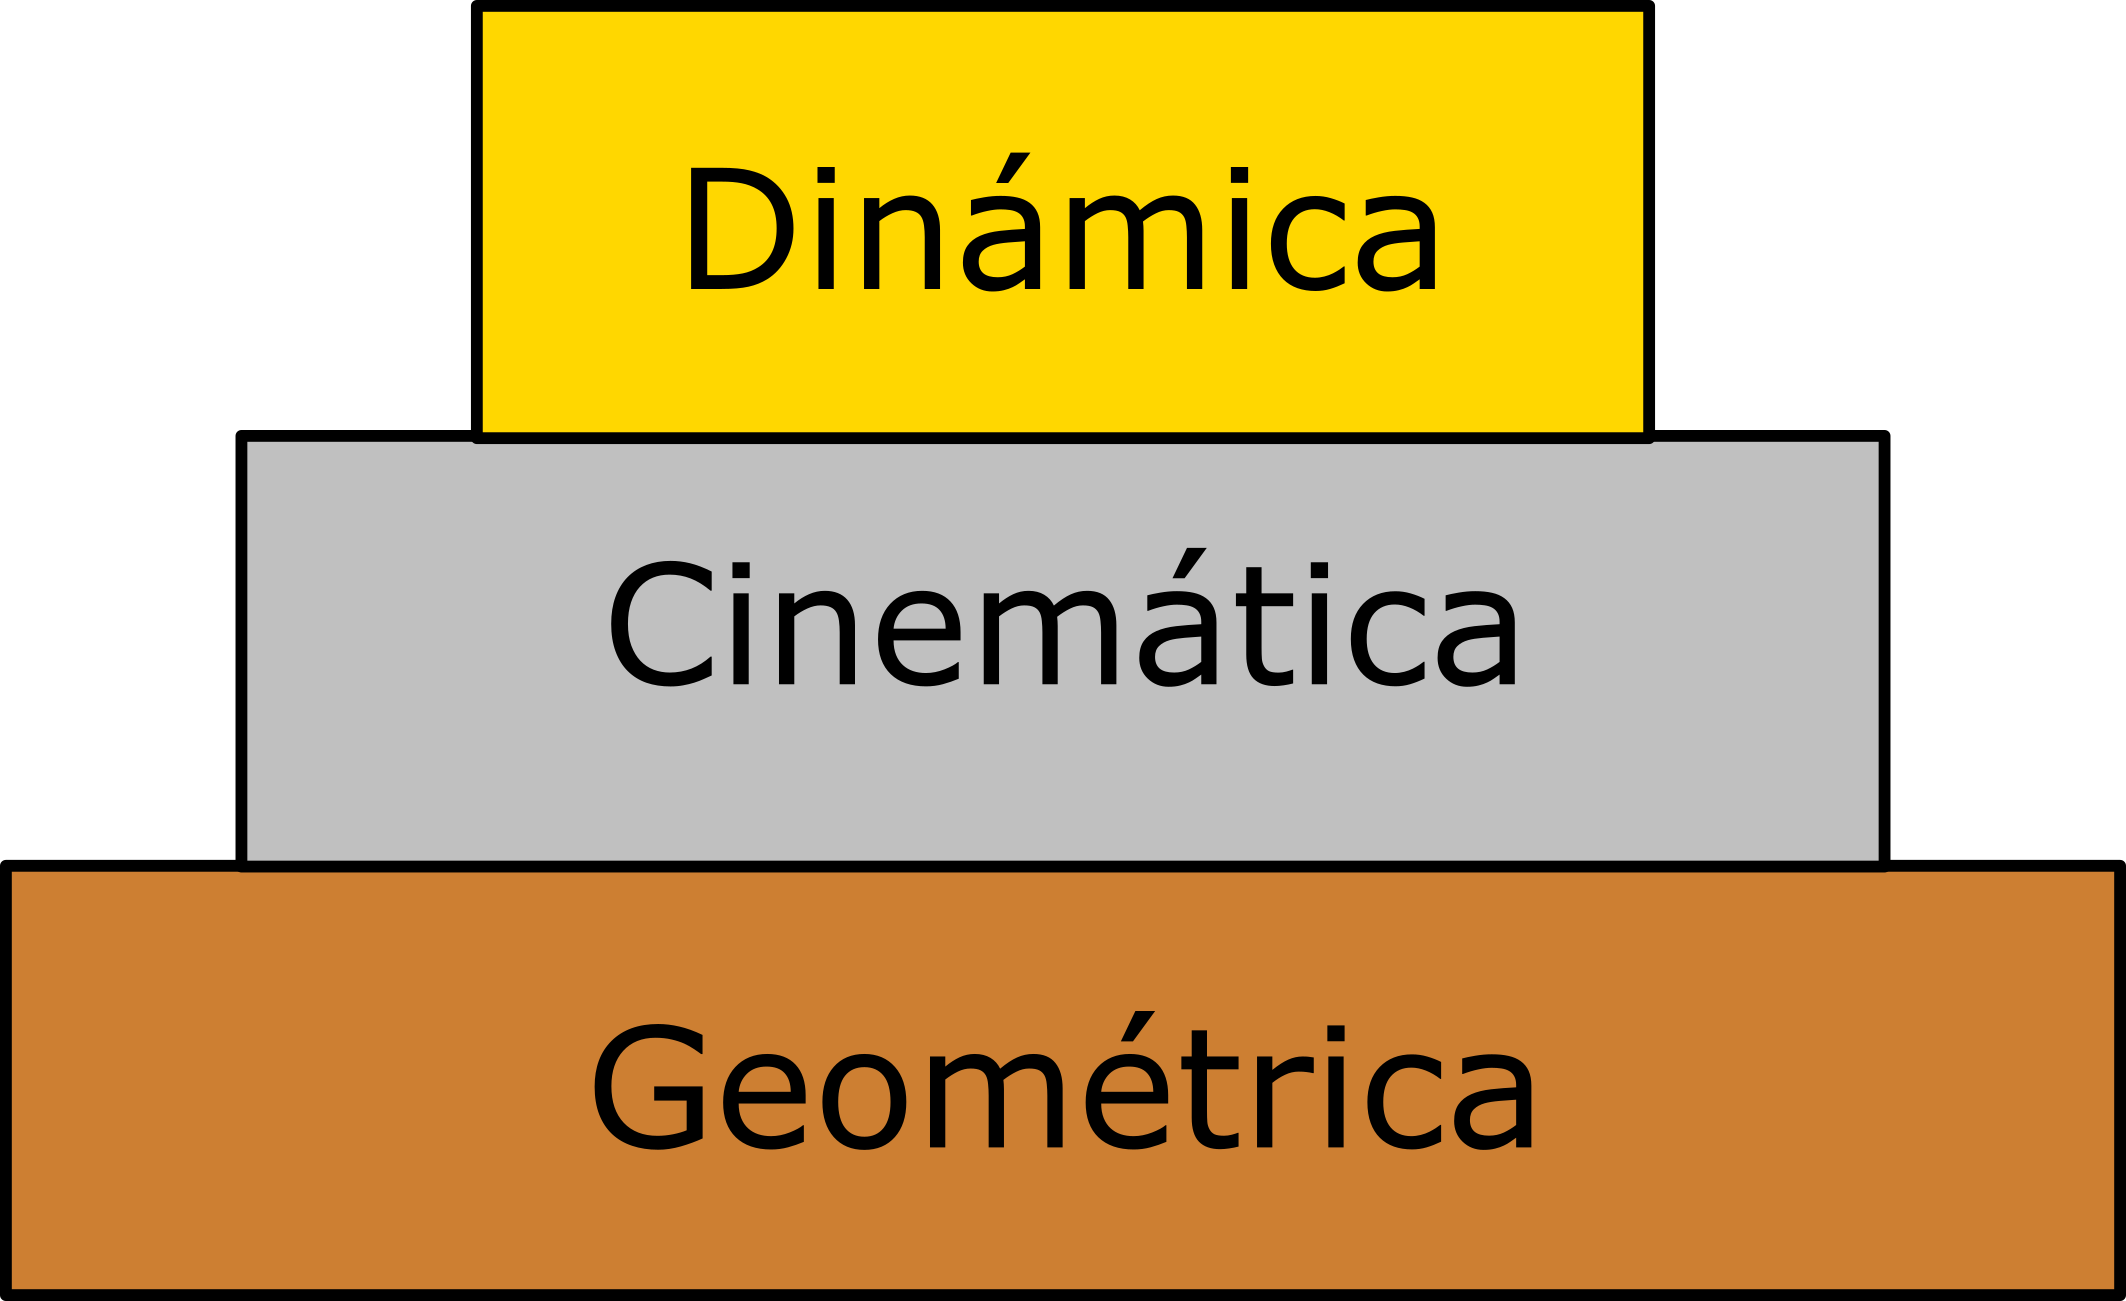
\includegraphics[width=0.8\textwidth]{Figures/grados_sim.png}
\end{columns}
\end{frame}
%%%%%%%%%%%%%%%%%%%%%%%%%%%%%%%%%%%%%%%%%%%%%%%%%%%%%%%%%%%%%%%%%%%%%%%%%%%%%%
\begin{frame}
\frametitle{Similitud geométrica}


    \textbf{El modelo y el prototipo deben poseer la misma forma geométrica. El
tamaño del modelo puede ser modificado mediante algún factor de escala.}

\vspace{0.2cm}

Para cumplir con este tipo de similitud se requiere que:

    \begin{itemize}
\item
  Todas las dimensiones del modelo tengan la misma escala lineal con las
  dimensiones del prototipo. 
\item
  Todos los ángulos se conserven (los ángulos en modelo y prototipo sean
  iguales). 
\item
  Todas las direcciones de flujo se conserven. 
\item
  La orientación del modelo y del prototipo con respecto a sus
  alrededores deben ser idénticas. 
\end{itemize}

\end{frame}
%%%%%%%%%%%%%%%%%%%%%%%%%%%%%%%%%%%%%%%%%%%%%%%%%%%%%%%%%%%%%%%%%%%%%%%%%%%%%%
\begin{frame}
\frametitle{Similitud cinemática}

  \textbf{La velocidad en cualquier punto en el flujo del modelo debe ser
proporcional a la velocidad en el punto correspondiente en el flujo del
prototipo (la escala debe ser la misma para todos los puntos)}. 

\vspace{0.2cm} 

Para
cumplir con este tipo de similitud se requiere que:

    \begin{itemize}
\item
  Exista semejanza geométrica. 
\item
  El escalamiento temporal debe tener la misma escala lineal que el
  escalamiento geométrico (\(L_m/L\)). 
\item
  Las velocidades que describen el movimiento del fluido en el modelo
  tienen la misma escala lineal con las velocidades del prototipo
  (\(V_m/V\)).
\end{itemize}

Nota: Existirá semejanza cinemática si partículas homólogas se
encuentran en puntos homólogos a tiempos homólogos.
\end{frame}
%%%%%%%%%%%%%%%%%%%%%%%%%%%%%%%%%%%%%%%%%%%%%%%%%%%%%%%%%%%%%%%%%%%%%%%%%%%%%%
\begin{frame}
\frametitle{Similitud dinámica}

    \textbf{Todas las fuerzas en el flujo del modelo se escalan por un factor
constante a las fuerzas correspondientes el el flujo del prototipo.}

\vspace{0.2cm}

 Para cumplir con este tipo de similitud se requiere que:

    \begin{itemize}
\item
  Exista semejanza geométrica. Se debe cumplir con todos los
  requerimientos para este tipo de similitud.
\item
  Exista semejanza cinemática. Se debe cumplir con todos los
  requerimientos para este tipo de similitud.
\item
  El escalamiento de las fuerzas debe tener la misma escala lineal que
  los escalamientos geométrico y cinemático. 
\item
  Las fuerzas en el modelo tienen la misma escala lineal con las fuerzas
  del prototipo.
\end{itemize}
\end{frame}
%%%%%%%%%%%%%%%%%%%%%%%%%%%%%%%%%%%%%%%%%%%%%%%%%%%%%%%%%%%%%%%%%%%%%%%%%%%%%%
\begin{frame}
\frametitle{Similitud dinámica en flujos de fluidos}

    \textbf{La similitud dinámica corresponde a más restrictivo de los tres tipos,
ya que requiere de los otros dos tipos de similitud} (de igual forma, la
similitud cinemática es más restrictiva que la geométrica). De manera
general, dependiendo del tipo de flujo, lograremos la similitud dinámica
cuando (suponiendo que se posee similitud geométrica):
\vspace{0.5cm}

    \begin{itemize}
\item
  \textbf{Flujo compresible}: \(\operatorname{Re}\), \(\operatorname{Ma}\) y
  \(k=c_p/c_v\) son iguales para modelo y prototipo.
\item
  \textbf{Flujo incompresible sin superficie libre}: \(\operatorname{Re}\) es
  igual para modelo y prototipo.
\item
  \textbf{Flujo incompresible con superficie libre}: \(\operatorname{Re}\) y
  \(\operatorname{Fr}\) deben ser iguales para modelo y prototipo.
  Dependiendo del caso, también \(\operatorname{We}\)
\end{itemize}

\end{frame}
%%%%%%%%%%%%%%%%%%%%%%%%%%%%%%%%%%%%%%%%%%%%%%%%%%%%%%%%%%%%%%%%%%%%%%%%%%%%%%
\subsection{Similitud incompleta}
\begin{frame}
\frametitle{Similitud incompleta}
 Consideremos el estudio del flujo de un fluido en un canal abierto. Supongamos que  este flujo puede sercaracterizado mediante el número de Reynolds ($\operatorname{Re}$) y el número de Froude ($\operatorname{Fr}$). Para lograr la similitud din\'amica se requiere:

$$\operatorname{Fr}_m = \operatorname{Fr}_p \quad\land\quad \operatorname{Re}_m = \operatorname{Re}$$

 La similitud del \textbf{n\'umero de Froude} requiere:

$$\operatorname{Fr}_m = \operatorname{Fr} \qquad \Rightarrow \qquad {\color{red}{\frac{V_m}{\sqrt{g_m L_m}} = \frac{V}{\sqrt{gL}}}}$$

 Ya que tanto modelo y prototipo son operados en el mismo campo gravitacional, la escala de velocidad es:

$$\color{blue}{\frac{V_m}{V} = \sqrt{\frac{L_m}{L}}=\sqrt{\lambda_L}}$$

\end{frame}
%%%%%%%%%%%%%%%%%%%%%%%%%%%%%%%%%%%%%%%%%%%%%%%%%%%%%%%%%%%%%%%%%%%%%%%%%%%%%%
\begin{frame}
La similitud del \textbf{n\'umero de Reynolds} requiere:

$$
\operatorname{Re}_m = \operatorname{Re} \qquad \Rightarrow 
\qquad {\color{red}{\frac{\rho_m V_m L_m}{\mu_m} = \frac{\rho V L}{\mu}}}$$

 La escala de velocidad en base a este n\'umero es:

$$\color{magenta}{\frac{V_m}{V} = \frac{\mu_m}{\mu} \frac{\rho}{\rho_m} \frac{L}{L_m}}$$

 Considerando que la escala de velocidad tambi\'en debe ser determinada por el número de Froude $\operatorname{Fr}$:

$${\color{magenta}{\frac{\mu_m}{\mu} \frac{\rho}{\rho_m} \frac{L}{L_m}}} = {\color{blue}{\sqrt{\frac{L_m}{L}}}} = \sqrt{\lambda_m}$$

 De esta forma:

$$\frac{\mu_m / \rho_m}{\mu/\rho} = \frac{\nu_m}{\nu} = \left( \lambda_m\right)^{3/2}$$

\end{frame}
%%%%%%%%%%%%%%%%%%%%%%%%%%%%%%%%%%%%%%%%%%%%%%%%%%%%%%%%%%%%%%%%%%%%%%%%%%%%%%
\begin{frame}

La expresi\'on:

$$\frac{\nu_m}{\nu} = \left( \lambda_m\right)^{3/2}$$

Establece que para lograr \textbf{similitud din\'amica}, se debe utilizar un fluido cuya viscosidad cinem\'atica $\nu_m$ cumpla:

$$\nu_m = \nu \left( \lambda_m\right)^{3/2}$$

\textbf{\color{red}{Lo cual puede ser muy dif\'icil (o imposible!).}} 

\vspace{0.2cm}

\textbf{Por ejemplo:} Supongamos que deseamos estudiar el flujo de agua en un canal abierto. Para esto, decidimos crear un modelo en una escala de $1/8$. La viscosidad cinemática del fluido a utilizar en el modelo debiese ser $\nu_m = \nu_{\text{agua}}\left(1/8\right)^{3/2} = 0.0442\, \nu_{\text{agua}}$. Entones, deberemos emplear un líquido que cumpla con este requerimiento (¡pero antes deberemos encontrarlo!).
\end{frame}
%%%%%%%%%%%%%%%%%%%%%%%%%%%%%%%%%%%%%%%%%%%%%%%%%%%%%%%%%%%%%%%%%%%%%%%%%%%%%%

\end{document}